% Options for packages loaded elsewhere
\PassOptionsToPackage{unicode}{hyperref}
\PassOptionsToPackage{hyphens}{url}

%=========
% BEAMER CLASS OPTIONS
%=========
\documentclass[%
  9pt,
  spanish, % Set language for babel
  ignorenonframetext,
  aspectratio=169, % Set aspect ratio (default: 16:9)
]{beamer}

% ==========
% MAIN PACKAGES
% ==========
\usepackage{tikz}
\usepackage{etoolbox}
\usepackage{setspace}

% Set the language
\usepackage[shorthands=off,%
main=spanish]{babel}

\usepackage{pgfpages}

% ==========
% CAPTIONS FOR FIGURES
% ==========
\setbeamertemplate{caption}[numbered]
\setbeamertemplate{caption label separator}{: }
\setbeamercolor{caption name}{fg=normal text.fg}
\beamertemplatenavigationsymbolsempty

% =========
% BEAMER OPTIONS
% =========

% Prevent slide breaks in the middle of a paragraph
\widowpenalties 1 10000
\raggedbottom

% Templates for slide section titles
% We need to design the 'part' slide, which is a special slide in beamer
\setbeamertemplate{part page}{
  \centering
  \begin{beamercolorbox}[sep=16pt,center]{part title}
    \usebeamerfont{part title}\insertpart\par
  \end{beamercolorbox}
}
\AtBeginPart{
  \frame{\partpage}
}

% Define the section and subsection slides
\setbeamertemplate{section page}{
  \centering
  \begin{beamercolorbox}[sep=12pt,center]{part title}
    {\usebeamerfont{section name}\usebeamercolor[fg]{section name}}
    {\usebeamerfont{section title}\insertsection\par}
  \end{beamercolorbox}
}
\AtBeginSubsection{
  \frame{\subsectionpage}
}


\usepackage{ifxetex,ifluatex}
\ifnum 0\ifxetex 1\fi\ifluatex 1\fi=0 % if pdftex
\usepackage[T1]{fontenc}
\usepackage[utf8]{inputenc}
\usepackage{textcomp} % provide euro and other symbols
\fi

% =========
% DEFAULT SLIDE DESIGN
% =========

% Sets the slide theme. Default: Berlin %
\usetheme{Berlin}
\makeatletter
\def\beamer@writeslidentry{\clearpage\beamer@notesactions}
\makeatother

% Slide text size
\setbeamersize{text margin left=3em, text margin right=3em}

\setlength{\emergencystretch}{3em} % prevent overfull lines

% Head Line (Section bar on the top of each slide)
\setbeamercolor{headline}{bg=main-color!50!black,fg=white}
\setbeamertemplate{headline}{%
  \begin{beamercolorbox}[wd=\paperwidth,ht=4ex,dp=0pt,left]{headline}%
    \hspace*{6pt}\vbox to4ex{\vfil\vspace{1pt}\insertsectionhead\vfil}
  \end{beamercolorbox}
}

% Title of the slide
\setbeamertemplate{frametitle}{%
  \nointerlineskip % Avoid a space before the box
  \begin{beamercolorbox}[wd=\paperwidth,ht=4ex,dp=0pt,left]{frametitle}%
    \hspace*{6pt}\vbox to4ex{\vfil\vspace{1pt}\insertframetitle\vfil}
  \end{beamercolorbox}
}

% Foot line (Bottom part of the slide)
\setbeamercolor{footline}{bg=main-color,fg=white}
\setbeamertemplate{footline}{%
  \nointerlineskip % Avoid a space before the box
  \begin{beamercolorbox}[wd=\paperwidth,ht=4ex,dp=0pt,left]{footline}%
    \vbox to 4ex {\vfil\vspace{1pt}%
      \hbox to \paperwidth{%
      \hspace{6pt}\insertshorttitle \hfill \insertauthor\hspace{6pt}}%
    \vfil}
  \end{beamercolorbox}
}

% ============
% COLORS AND COLOR PALETTE
% ============

\usepackage[dvipsnames]{xcolor} % Allows using colors

% Color palette: Catpuccin Latte
\definecolor{main-color}{HTML}{1e66f5} % Used in top and bottom of
% slides, itemize dots, and other structure

% Used for highlights
\definecolor{blue}{HTML}{1e66f5}
\definecolor{green}{HTML}{40a02b}
\definecolor{red}{HTML}{d20f39}
\definecolor{gray}{HTML}{555566}
\definecolor{lightgray}{HTML}{808080}

% Apply the main color to highlighted elements
\setbeamercolor{structure}{fg=main-color} % itemize, enumerate, etc

% Use upquote if available, for straight quotes in verbatim environments
\IfFileExists{upquote.sty}{\usepackage{upquote}}{}
\IfFileExists{xurl.sty}{\usepackage{xurl}}{} % add URL line breaks if available

% Define hyperlinks and bookmarks
\usepackage{bookmark}
\usepackage{hyperref}
\hypersetup{
  pdftitle={Objetividad fuerte y neutralidad en la ciencia de la emoción},
  pdflang={es},
  hidelinks,
}

% Sets the geometry

% Sets spacing for columns
\BeforeBeginEnvironment{columns}{\vspace{0.75em}}
\AfterEndEnvironment{columns}{\vspace{0.75em}}
\setlength{\columnsep}{1ex}

% ===========
% FONTS
% ===========

% Use custom font
\usefonttheme{professionalfonts}

% Load and set math fonts
\usepackage{amssymb,amsmath} % Must be loaded before mathspec
\usepackage{mathspec}
\makeatletter % undo the wrong changes made by mathspec, see
% https://tex.stackexchange.com/questions/85696/what-causes-this-strange-interaction-between-glossaries-and-amsmath
\let\RequirePackage\original@RequirePackage
\let\usepackage\RequirePackage
\makeatother

\setmathsfont(Latin,Digits,Greek){TeX Gyre Bonum}

% Set default text font
\usepackage{fontspec}
\setsansfont{Lato}

% Use FontAwesome for symbols
\usepackage{fontawesome5}

\makeatletter
\renewcommand{\tiny}{\@setfontsize\tiny{5pt}{5pt}} % {font size}{line spacing}
\makeatother

% ============
% TABLES
% ============
\usepackage{tabularx} % Helps with formatting tables

% ============
% GRAPHICS: Helps use images in slides
% ============

% ===========
% LISTS
% ===========
\providecommand{\tightlist}{}

\setbeamertemplate{itemize items}[circle]
\setbeamertemplate{enumerate items}[default]

\setbeamertemplate{itemize/enumerate subbody begin}{\vspace{0cm}}
\setbeamertemplate{itemize/enumerate subbody end}{\vspace{0cm}}

% ===========
% QUOTES
% ===========
\usepackage{csquotes}

\addtobeamertemplate{quote begin}{\vskip1ex}{}

% Don't italicize quotes
\setbeamerfont{quote}{shape=\upshape}
\setbeamercolor{quote}{fg=gray}

% Blockquote colors
\definecolor{blockquote-border}{RGB}{221,221,221}
\definecolor{blockquote-text}{RGB}{89,89,89}

% Blockquote box
\usetikzlibrary{arrows.meta}
\usetikzlibrary{positioning}
\usetikzlibrary{decorations.pathreplacing}
\usetikzlibrary{fit}
\usepackage[framemethod=TikZ]{mdframed}
\surroundwithmdframed[%
  linewidth=0.5pt,%
  linecolor=gray!50!white,
  skipabove=1em,%
  skipbelow=2em,%
  leftmargin=0.5em,%
  rightmargin=1em,%
  innerleftmargin=-1em,%
  innerrightmargin=-1em%,
  innertopmargin=0.2em,%
  innerbottommargin=0.5em,%
roundcorner=5pt]{quote}

\setbeamertemplate{blocks}[rounded][shadow=false]

\setbeamercolor{block body example}{bg=green!10!white}
\setbeamercolor{block title example}{bg=green!50!black, fg=white}

\setbeamercolor{block body}{bg=white}
\setbeamercolor{block title}{bg=white,fg=main-color}

% Paragraphs
\setlength\parskip{0.5\baselineskip}
\linespread{1.15}\selectfont % <---

% ===========
% BIBLIOGRAPHY
% Defaults:
% - Style: APA
% - No DOI
% - No URL
% ===========

\usepackage[
  style=apa,
  apamaxprtauth=2,
  doi=false,
  url=false,
  backend=biber,
]{biblatex}

\addbibresource{Brasil.bib}

\renewcommand*{\bibfont}{\tiny} % or \tiny, \scriptsize, etc.
\setlength{\bibhang}{0.5em} % Adjust this value (default is usually 1.5em)

% Custom bibliography reference command, we use it sometimes in class
\newcommand{\cit}[1]{\newline {\footnotesize \textcolor{lightgray}{(#1)}}}

% Define bibliography appearance
\setbeamertemplate{bibliography item}{\insertbiblabel}
\setbeamercolor{bibliography entry author}{parent=palette primary}
\setbeamercolor{bibliography entry title}{fg=black}
\setbeamercolor{bibliography entry location}{fg=black}
\setbeamercolor{bibliography entry note}{fg=black}

%\usepackage{caption}
%\captionsetup[figure]{labelformat=empty}% redefines the caption
% setup of the figures environment in the beamer class.

% Title slide template
\setbeamertemplate{title page}{
  \setstretch{1}
  I Congresso Latino-Americano de Ciências Afetivas\\
  \vspace{6pt}
  {\LARGE\bfseries
    \inserttitle
  }\par\vskip1em
  {\large
    \insertauthor
  }\par
  {\small
    Departamento de Filosofía\\
    Universidad Alberto Hurtado
  }\par

  {\footnotesize \insertdate}
}

% Footnote template
\renewcommand{\thefootnote}{\color{lightgray}[\arabic{footnote}]}
\renewcommand\footnoterule{}
\setbeamertemplate{footnote}{%
  \parindent 0em%              % Remove indentation
  \color{lightgray}%
  \tiny
  \makebox[2em][l]{\normalfont\thefootnote}\insertfootnotetext\par%
}

\setcounter{secnumdepth}{-\maxdimen} % remove section numbering

% Use ~ as negation
\renewcommand{\lnot}{\mathord{\sim}}

% ===========
% CUSTOM COLORED BOXES
% ===========
\usepackage[most]{tcolorbox}

\newtcolorbox{alertbox}[1]{%
  colback=red!5!white,%
  colframe=red!75!black,%
  left=1ex,%
  right=1ex,%
  top=0.5ex,%
  title={#1}
}




% ===========
% PRESENTATION TITLE AND METADATA
% ===========
\title{Objetividad fuerte y neutralidad en la ciencia de la emoción}

\author{Juan R. Loaiza}

\date{12 de agosto de 2025}

\institute{Departamento de Filosofía · Universidad Alberto Hurtado}

% ===========
% DOCUMENT START
% ===========
\begin{document}

% Frontmatter

% Title page
\frame{\titlepage}

% Table of contents, lists of tables and figures

% Set line spacing for main content
\setstretch{1.15}

% Main content

\section{Introducción}\label{introducciuxf3n}

\begin{frame}{Introducción}
  Hay varias ciencias que nos dan conocimiento sobre las emociones.

  \begin{center}

    \begin{tabular}{cccc}
      
\includegraphics[height=10em]{fig1.1_psicologia.png} &
      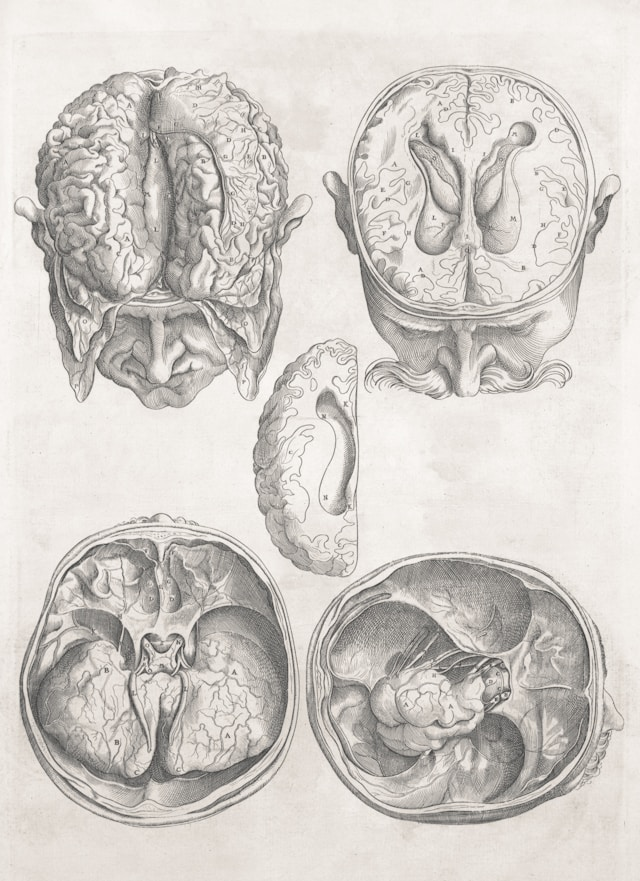
\includegraphics[height=10em]{fig1.2_neurociencia.jpg} &
      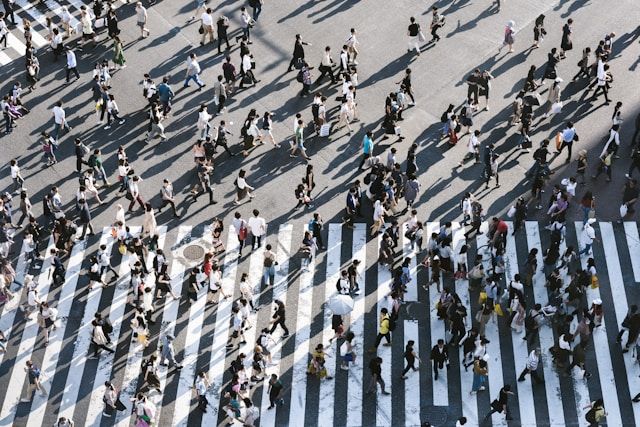
\includegraphics[height=10em]{fig1.3_socsci.jpg} &
      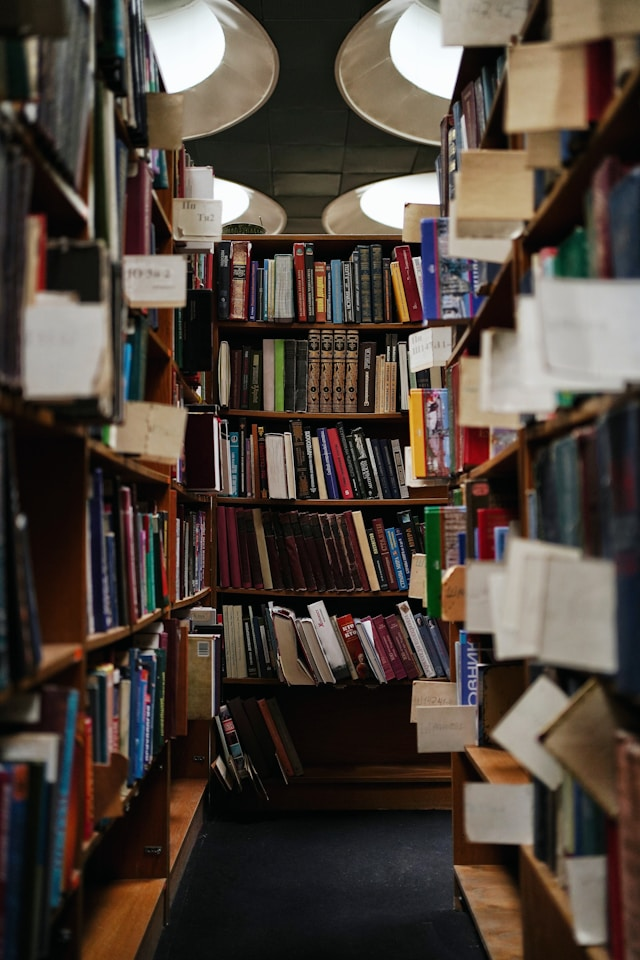
\includegraphics[height=10em]{fig1.4_linguistics.jpg} \\
      Psicología & Neurociencia & Ciencias Sociales & Lingüística \\
    \end{tabular}
  \end{center}
\end{frame}

\begin{frame}{Pregunta y tesis}
  \phantomsection\label{pregunta-y-tesis}
  ¿Es nuestro \textbf{conocimiento científico} sobre las emociones
  \textbf{objetivo}? \pause

  \textbf{Tesis}: El conocimiento científico sobre las emociones falla en
  varios criterios de objetividad. \pause

  \begin{itemize}
      \tightlist
    \item
      La producción de conocimiento no es robusta. \pause
    \item
      No es una ciencia crítica de los valores que la influyen. \pause
    \item
      No hay mecanismos de acuerdo teórico entre investigadores/as. \pause
  \end{itemize}

  Si queremos aspirar a la objetividad en la ciencia de la emoción,
  debemos atender varios aspectos sociales de las comunidades que la
  conforman.
\end{frame}

\begin{frame}{Plan}
  \phantomsection\label{plan}
  \begin{enumerate}
      \tightlist
    \item
      ¿Qué es la objetividad en la ciencia?
    \item
      ¿Es la ciencia de la emoción objetiva?

      \begin{enumerate}
          \tightlist
        \item
          Producción de conocimiento
        \item
          Ciencia y valores
        \item
          Acuerdo teórico
      \end{enumerate}
    \item
      Conclusión: en búsqueda de la objetividad
  \end{enumerate}
\end{frame}

\section{Objetividad en la ciencia}\label{objetividad-en-la-ciencia}

\begin{frame}{Respuestas clásicas a la objetividad}
  \phantomsection\label{respuestas-cluxe1sicas-a-la-objetividad}
  Tradicionalmente, se asociaba objetividad con dos criterios:
  \footnote[frame]{\fullcite[][]{Carnap1928}} \pause

  \begin{columns}[T,onlytextwidth]
    \begin{column}{0.48\textwidth}
      \textbf{Independencia de la mente} \pause

      El conocimiento científico es ``objetivo'' si no depende de la mente del
      investigadores/as. \pause

      \begin{itemize}
          \tightlist
        \item
          No depende de deseos del/de la investigador/a. \pause
        \item
          No es manipulable por la intención.
      \end{itemize}
    \end{column}

    \begin{column}{0.48\textwidth}
      \pause

      \textbf{Intersubjetividad}

      \pause

      El conocimiento científico es objetivo si puede ser validado por
      otros/as investigadores/as.

      \pause

      \begin{itemize}
          \tightlist
        \item
          Hay criterios públicos de corrección. \pause
        \item
          Hay mecanismos de discusión y acuerdo.
      \end{itemize}
    \end{column}
  \end{columns}

  \pause

  «Objetividad» también se ha asociado a \textbf{neutralidad} y
  \textbf{realidad}.
\end{frame}

\begin{frame}{Contra la neutralidad}
  \phantomsection\label{contra-la-neutralidad}
  Entender la objetividad como neutralidad es
  limitante.\footnote[frame]{\fullcite[][]{Longino1990a}}
  \footnote[frame]{\fullcite[][]{Harding1995}}

  \begin{columns}[T,onlytextwidth]
    \begin{column}{0.48\textwidth}
      \pause

      Hay valores que influyen en las decisiones científicas.

      \pause

      \begin{itemize}
          \tightlist
        \item
          Selección de problemas y prioridades. \pause
        \item
          Planteamiento de preguntas. \pause
        \item
          Elección de métodos y análisis.
      \end{itemize}
    \end{column}

    \begin{column}{0.48\textwidth}
      \pause

      No atender a estos valores no implica que no existan.

      \pause

      \begin{itemize}
          \tightlist
        \item
          Invisibiliza su acción. \pause
        \item
          Refuerza valores dominantes.
      \end{itemize}
    \end{column}
  \end{columns}

  \pause

  \textbf{Consecuencia:} Bajo los análisis tradicionales, ninguna ciencia
  es objetiva.
\end{frame}

\begin{frame}{¿Y por qué la objetividad?}
  \phantomsection\label{y-por-quuxe9-la-objetividad}
  ¿Por qué querríamos ciencias ``objetivas''?

  \pause

  \begin{itemize}
      \tightlist
    \item
      Necesitamos estándares de justificación y validación del conocimiento.
      \pause
    \item
      El conocimiento \textbf{no} debe ser \textbf{arbitrario}.
  \end{itemize}

  \pause

  La arbitrariedad en el conocimiento tiene al menos dos consecuencias
  indeseables:

  \pause

  \begin{itemize}
      \tightlist
    \item
      Nos aleja de conocimiento verdadero o útil. \pause
    \item
      Permite manipulaciones peligrosas del ``conocimiento científico''.
  \end{itemize}

  \pause

  \textbf{Propuesta:} Buscar criterios operacionales (aplicables) claros
  de ``objetividad''.
\end{frame}

\begin{frame}{El análisis de Douglas}
  \phantomsection\label{el-anuxe1lisis-de-douglas}
  \textcite[][]{Douglas2004}\footnote[frame]{\fullcite{Douglas2004}}
  distingue tres modos y ocho sentidos de «objetividad»: \pause

  \begin{columns}[T,onlytextwidth]
    \begin{column}{0.33\textwidth}
      \textbf{Producción de conocimiento}

      \pause

      Manipulabilidad

      \pause

      Convergencia

      \pause
    \end{column}

    \begin{column}{0.33\textwidth}
      \textbf{Procesos de razonamiento}

      \pause

      Separación de valores

      \pause

      Ser libre de valores

      \pause

      Ser neutral a los valores

      \pause
    \end{column}

    \begin{column}{0.33\textwidth}
      \textbf{Procesos sociales}

      \pause

      Procedimentalización

      \pause

      Concordancia (consenso)

      \pause

      Interactividad (argumentatividad)
    \end{column}
  \end{columns}

  \pause

  Douglas sostiene que son sentidos irreductibles. No haremos tal
  suposición.

  \pause

  \textbf{Propuesta}: Evaluar en qué criterios las ciencias afectivas son
  más objetivas.
\end{frame}

\section{Producción de
conocimiento}\label{producciuxf3n-de-conocimiento}

\begin{frame}{Manipulabilidad}
  \phantomsection\label{manipulabilidad}
  El conocimiento científico es objetivo si podemos manipular o intervenir
  en los fenómenos de manera consistente.

  \pause

  \begin{itemize}
      \tightlist
    \item
      e.g.: Intervenciones experimentales
  \end{itemize}

  \pause

  \begin{columns}[T,totalwidth=0.8\textwidth]
    \begin{column}{0.48\textwidth}
      \textbf{Replicabilidad}

      Podemos hacer nuevamente el experimento y obtener los mismos resultados.
    \end{column}

    \begin{column}{0.48\textwidth}
      \textbf{Reproducibilidad}

      Podemos hacer el mismo análisis con los mismos datos y obtener los
      mismos resultados.
    \end{column}
  \end{columns}

  \pause

  En el caso de las emociones, podemos revisar los estudios sobre
  \textbf{inducción de emociones}.
\end{frame}

\begin{frame}{Manipulabilidad}
  \phantomsection\label{manipulabilidad-1}
  Algunos estudios sugieren que podemos inducir emociones específicas en
  ciertas
  condiciones.\footnote[frame]{\fullcite[][]{Schachter1962}}
  \footnote[frame]{\fullcite[][]{Lobbestael2008}}
  \footnote[frame]{\fullcite[][]{Feinstein2011}}
  \pause

  Otros estudios sugieren lo contrario.

  \pause

  \begin{itemize}
      \tightlist
    \item
      La inducción de emociones con música
      \footnote[frame]{\fullcite[][]{Etzel2006}}, películas
      \footnote[frame]{\fullcite[][]{Fernandez-Aguilar2020}} o recuento
      autobiográfico \footnote[frame]{\fullcite[][]{McGinley2017}} no
      permite inducir emociones específicas. \pause
    \item
      El método de inducción cambia variables
      autonómicas.\footnote[frame]{\fullcite[][]{Mills2014}}
  \end{itemize}

  \pause

  No parecemos tener métodos robustos de manipulación de emociones en
  contextos experimentales.
\end{frame}

\begin{frame}{Convergencia}
  \phantomsection\label{convergencia}
  El conocimiento científico es objetivo si podemos \textbf{observar lo
  mismo} bajo distintos métodos.

  \pause

  En el caso de las emociones, tenemos distintas
  dimensiones:\footnote[frame]{\fullcite[][]{Scherer2005}}

  \pause

  \begin{itemize}
      \tightlist
    \item
      Mecanismos neurológicos \pause
    \item
      Patrones fisiológicos \pause
    \item
      Expresiones faciales \pause
    \item
      Comportamientos y tendencias a la acción \pause
    \item
      Fenomenología
  \end{itemize}
\end{frame}

\begin{frame}{Convergencia}
  \phantomsection\label{convergencia-1}
  ¿Qué cuenta como ``\textbf{observar lo mismo}''?

  \pause

  Hay demasiada \textbf{variabilidad} en las respuestas emocionales.

  \pause

  \begin{itemize}
      \tightlist
    \item
      No hay consistencia o especificiar neuronal o
      fisiológica.\footnote[frame]{\fullcite[][]{Barrett2006}}
      \footnote[frame]{\fullcite[][]{Lindquist2012a}}
      \pause
    \item
      Las expresiones faciales no son específicas a cada
      emoción.\footnote[frame]{\fullcite[][]{Barrett2019}} \pause
    \item
      Las conductas son altamente contextuales y
      variadas.\footnote[frame]{\fullcite[][]{Barrett2022}} \pause
    \item
      No hay protocolos de comparación fenomenológica.
  \end{itemize}

  \pause

  No hay criterios de individuación que permitan establecer convergencia
  entre distintos métodos.\footnote[frame]{\fullcite[][]{Loaiza2021}}
\end{frame}

\section{Ciencia de las emociones y
valores}\label{ciencia-de-las-emociones-y-valores}

\begin{frame}{Los roles de los valores en la ciencia}
  \phantomsection\label{los-roles-de-los-valores-en-la-ciencia}
  Hay varios sentidos en que la ciencia puede ser «objetiva» en cuanto
  cómo operan los valores. \pause

  \begin{columns}[T,onlytextwidth]
    \begin{column}{0.3\textwidth}
      \textbf{Separación de los valores}

      \pause

      Los valores no reemplazan la evidencia.

      \pause

      \begin{itemize}
          \tightlist
        \item
          Solo se aceptan consideraciones de valor ante subdeterminación por la
          evidencia. \pause
      \end{itemize}
    \end{column}

    \begin{column}{0.3\textwidth}
      \textbf{Libertad de valores}

      \pause

      Los valores no juegan \emph{ningún} rol en la ciencia.

      \pause

      \begin{itemize}
          \tightlist
        \item
          Todo (preguntas, hipótesis, teorías) se decide por evidencia. \pause
      \end{itemize}
    \end{column}

    \begin{column}{0.3\textwidth}
      \textbf{Neutralidad de valores}

      \pause

      Las decisiones son neutrales relativo a un conjunto de valores.

      \pause

      \begin{itemize}
          \tightlist
        \item
          No se toman decisiones circulares o radicales.
      \end{itemize}
    \end{column}
  \end{columns}
\end{frame}

\begin{frame}{¿Separación o libertad de valores?}
  \phantomsection\label{separaciuxf3n-o-libertad-de-valores}
  ¿Es la ciencia de la emoción \emph{libre} de valores? \pause ¡No! \pause

  \begin{itemize}
    \item
      Muchas decisiones sobre qué emociones hay (distinciones, criterios de
      identificación, etc.) presuponen marcos
      angloparlantes.\footnote[frame]{\fullcite[][]{Wierzbicka1999}}
      \footnote[frame]{\fullcite[][]{Wierzbicka2009b}}
      \pause

      \begin{itemize}
          \tightlist
        \item
          Las decisiones ontológicas no se toman por la evidencia, sino por
          estructuras sociales específicas. \pause
      \end{itemize}
    \item
      La psicología experimental en general está demasiado centralizada en
      poblaciones WEIRD.\footnote[frame]{\fullcite[][]{Henrich2010}} \pause
    \item
      La historia de la ciencia de las emociones está motivada por intereses
      éticos y políticos. \pause

      \begin{itemize}
          \tightlist
        \item
          La teoría de la expresión de Darwin está ligada al
          antiesclavismo.\footnote[frame]{\fullcite[][]{Ginnobili2025}} \pause
        \item
          El debate en torno a la universalidad de las emociones estuvo
          motivado por discusiones sobre el
          colonialismo.\footnote[frame]{\fullcite[][]{Ekman2009}}
      \end{itemize}
  \end{itemize}
\end{frame}

\begin{frame}{¿Debe la ciencia ser libre de valores?}
  \phantomsection\label{debe-la-ciencia-ser-libre-de-valores}
  Hay buenas razones por las que la ciencia no debe omitir el rol de los
  valores.

  \pause

  \begin{itemize}
      \tightlist
    \item
      \textcite[][]{Longino1990a}\footnote[frame]{\fullcite{Longino1990a}}
      nos recomienda someter los valores a escrutinio crítico y público.
      \pause
    \item
      \textcite[][]{Harding1995}\footnote[frame]{\fullcite{Harding1995}}
      sostiene que la objetividad depende de la explicitación pública de
      valores.
  \end{itemize}

  \pause

  La ciencia de la emoción no puede ignorar los valores (culturales,
  políticos y sociales) que la influyen.
\end{frame}

\section{Procesos sociales}\label{procesos-sociales}

\begin{frame}{Procedimentalidad}
  \phantomsection\label{procedimentalidad}
  El conocimiento científico es objetivo si los procedimientos tienen los
  mismos resultados sin importar quién los ejecute.

  \pause

  \begin{itemize}
      \tightlist
    \item
      e.g., El análisis cuantitativo debe dar el mismo resultado sin
      importar quién haga el cálculo.
  \end{itemize}

  \pause

  No hay estudios que se enfoquen en si los/las investigadores/as son
  intercambiables.

  \pause

  \begin{itemize}
      \tightlist
    \item
      Hay estudios que muestran efectos del/de la
      experimentador/a.\footnote[frame]{\fullcite[][]{Edlund2014}}
  \end{itemize}

  \pause

  Los protocolos de validación de instrumentos ayudan a evitar estos
  problemas.
\end{frame}

\begin{frame}{Concordancia (consenso)}
  \phantomsection\label{concordancia-consenso}
  El conocimiento científico objetivo es aquel frente al que hay acuerdo
  entre investigadores/as.\footnote[frame]{\fullcite[][]{Quine1954}}

  \pause

  Hay pocos acuerdos en la ciencia de la emoción.

  \pause

  \begin{itemize}
      \tightlist
    \item
      ¿Son las emociones discretas o difieren en grado? \pause
    \item
      ¿Debemos esperar correspondencias entre cada emoción y algún mecanismo
      neuronal o fisiológico? \pause
    \item
      ¿Difieren las emociones en aspectos únicamente corporales o también
      cognitivos?
  \end{itemize}
\end{frame}

\begin{frame}{Interactividad (argumentatibilidad)}
  \phantomsection\label{interactividad-argumentatibilidad}
  El conocimiento científico es objetivo si existen mecanismos para llegar
  a acuerdos.

  \pause

  No hay todavía criterios de acuerdo claros entre teorías de la emoción.

  \pause

  \begin{itemize}
      \tightlist
    \item
      Diferencias en criterios de individuación de las
      emociones.\footnote[frame]{\fullcite[][]{Loaiza2021}}
      \footnote[frame]{\fullcite[][]{Loaiza2024a}}
      \pause
    \item
      Distintas teorías difieren en cuáles son los fenómenos a
      explicar.\footnote[frame]{\fullcite[][]{Loaiza2022}} \pause
    \item
      No tenemos claro cuáles presuposiciones culturales inyectamos en el
      estudio de la emoción. \footnote[frame]{\fullcite[][]{Loaiza2025}}
  \end{itemize}

  \pause

  Aunque haya ``discusión'', no hay realmente diálogo entre teorías en
  ciencias afectivas.
\end{frame}

\section{Conclusiones}\label{conclusiones}

\begin{frame}{Diagnóstico}
  \phantomsection\label{diagnuxf3stico}
  Siguiendo varios criterios de objetividad, la ciencia de las emociones
  no es objetiva.

  \pause

  \begin{itemize}
      \tightlist
    \item
      No produce conocimiento de manera confiable \pause
    \item
      No es libre de valores \pause
    \item
      No hay mecanismos claros de acuerdo entre investigadores/as
  \end{itemize}

  \pause

  Esto no significa que debamos abandonar esta ciencia, pero sí que
  debemos pensar en cómo mejorarla.

  \pause

  Asumiendo que queremos una ciencia objetiva, \textbf{¿qué estrategias
  podemos implementar?}
\end{frame}

\begin{frame}{Recomendaciones}
  \phantomsection\label{recomendaciones}
  Los problemas de producción de conocimiento se deben a falta en
  decisiones epistémicas y ontológicas.

  \pause

  \begin{itemize}
      \tightlist
    \item
      ¿Cómo se \textbf{individuan} las emociones? (Ontología) \pause
    \item
      ¿Cómo se \textbf{identifican} las emociones? (Epistemología)
  \end{itemize}

  \pause

  Sobre la individuación, he sugerido aceptar un \textbf{funcionalismo}.

  \pause

  \begin{itemize}
      \tightlist
    \item
      Podemos individuar emociones por patrones abstractos de relaciones
      causales.
  \end{itemize}

  \pause

  Todavía tenemos pendiente la \textbf{identificación}.
\end{frame}

\begin{frame}{Recomendaciones}
  \phantomsection\label{recomendaciones-1}
  Muchos de los problemas con la objetividad de la ciencia de la emoción
  yacen en la organización de las comunidades científicas.

  \pause

  \begin{itemize}
      \tightlist
    \item
      Crítica a los valores \pause
    \item
      Criterios de acuerdo teórico (e.g., cuáles son los \emph{explananda})
  \end{itemize}

  \pause

  La ciencia de la emoción se beneficiaría de diseñar mejor sus
  comunidades científicas.

  \pause

  \begin{itemize}
      \tightlist
    \item
      Diversidad \pause
    \item
      Interdisciplinariedad \pause
    \item
      Estrategias de acuerdo
  \end{itemize}
\end{frame}

\begin{frame}{Recomendaciones}
  \phantomsection\label{recomendaciones-2}
  Revisar cómo se conforman las comunidades científicas nos ayuda a una
  ciencia más objetiva. \pause

  \begin{itemize}
      \tightlist
    \item
      División del trabajo cognitivo \pause
    \item
      Crítica y control de sesgos \pause
    \item
      Responsabilidad epistémica (\emph{accountability}). \pause
  \end{itemize}

  En la ciencia de la emoción, nos permite enfrentar dos desafíos: \pause

  \begin{itemize}
      \tightlist
    \item
      Explicitar presuposiciones (culturales, políticas, epistémicas) \pause
    \item
      Formar acuerdos teóricos y metodológicos
  \end{itemize}
\end{frame}

\section{}
\begin{frame}

  \centering
  {\LARGE
  \textbf{¡Muchas gracias!}}
  \vspace{-1em}

  \begin{minipage}[t]{0.7\textwidth}
    \begin{columns}
      \begin{column}{0.5\textwidth}
        \centering
        {
          
\includegraphics[height=10em]{qr_juanrloaizacom.pdf}

          Sitio web personal
        }
      \end{column}

      \begin{column}{0.5\textwidth}
        \centering
        {
          
\includegraphics[height=10em]{linkppt.pdf}

          Presentación
        }
      \end{column}
    \end{columns}
  \end{minipage}

  \setstretch{1}

  jloaiza@uahurtado.cl

  www.juanrloaiza.com

  www.santiagomindandcognition.cl

\end{frame}

% Bibliography slide
\begin{frame}[allowframebreaks]
  \frametitle{Bibliografía}
  \printbibliography
\end{frame}

\end{document}
